%% Los cap'itulos inician con \chapter{T'itulo}, estos aparecen numerados y
%% se incluyen en el 'indice general.
%%
%% Recuerda que aqu'i ya puedes escribir acentos como: 'a, 'e, 'i, etc.
%% La letra n con tilde es: 'n.

\chapter{Evaluaci\'on}
\section{Sistema de Visi\'on}
Utilizamos un robot del kit de robotica \textit{Robo Robo},  el cual fue programado para que se mueva aleatoriamente, ademas utilizamos una computadora Intel Core 2 Duo, bajo el Sistema Operativo Ubuntu 12.04. La camara que se utilizo fue una camara \textit{Logitech c210}, y se trabajo aproximadamente a 26 cuadros por segundo.\\
Se ha hecho pruebas con el sistema de visi\'on el cual encuentra los c\'irculos de las marcas sobre los robots, esto es realizado con la transformada de Hough utilizada del \textit{Opencv 2.4.6}, ademas se puede apreciar que al momento de capturar la imagen se muestra tambien la posicion actual del robot y la orientacion.\\
 Esto se hace para generar un archivo \textit{.dat} el cual servira como datos de entradas para nuestra red neuronal.
\begin{figure}
	\centering
	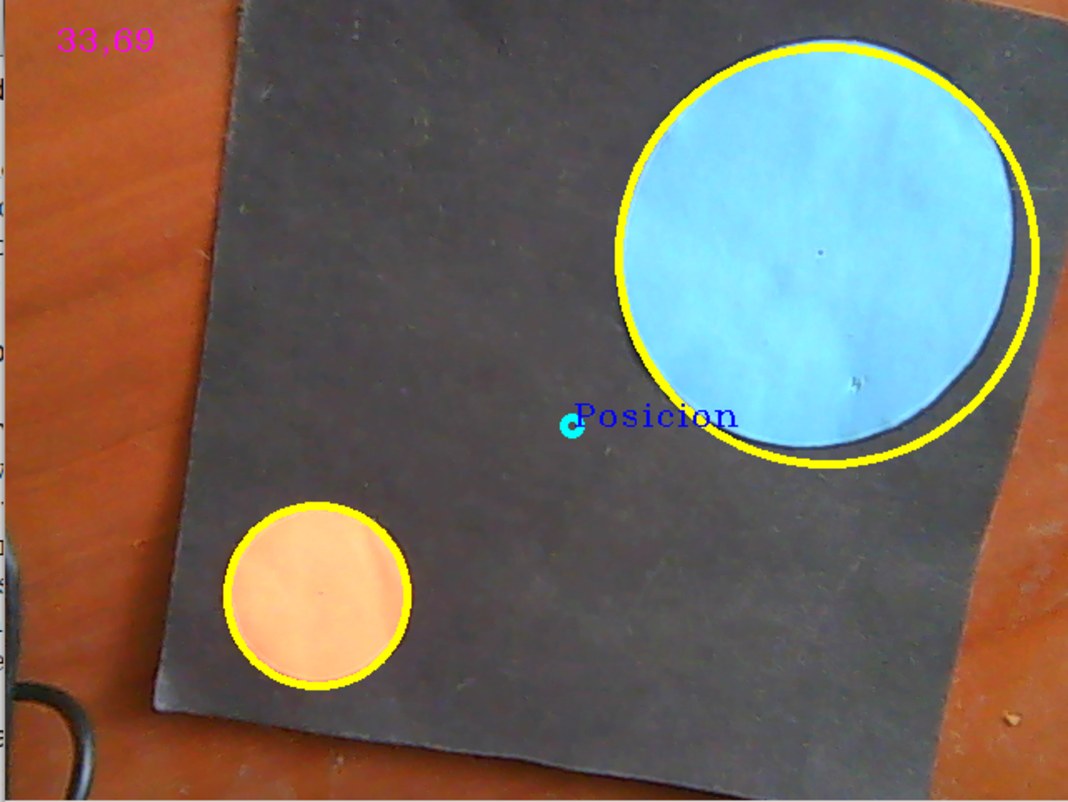
\includegraphics[width=2.5in]{visi.pdf}
	
	\caption{Ubicacion de los circulos}
	\label{fig_mar}
\end{figure}
\section{Seguimiento del Objeto}
Como  ya se menciono anteriormente utilizamos los archivos generados por el sistema de vision para nuestro algoritmo de seguimiento, al realizar las comparaciones sobre las salidas generadas por la red y las salidas entregadas por nosotros obtuvimos la la figura 5.2 :
\begin{figure}
	\centering
	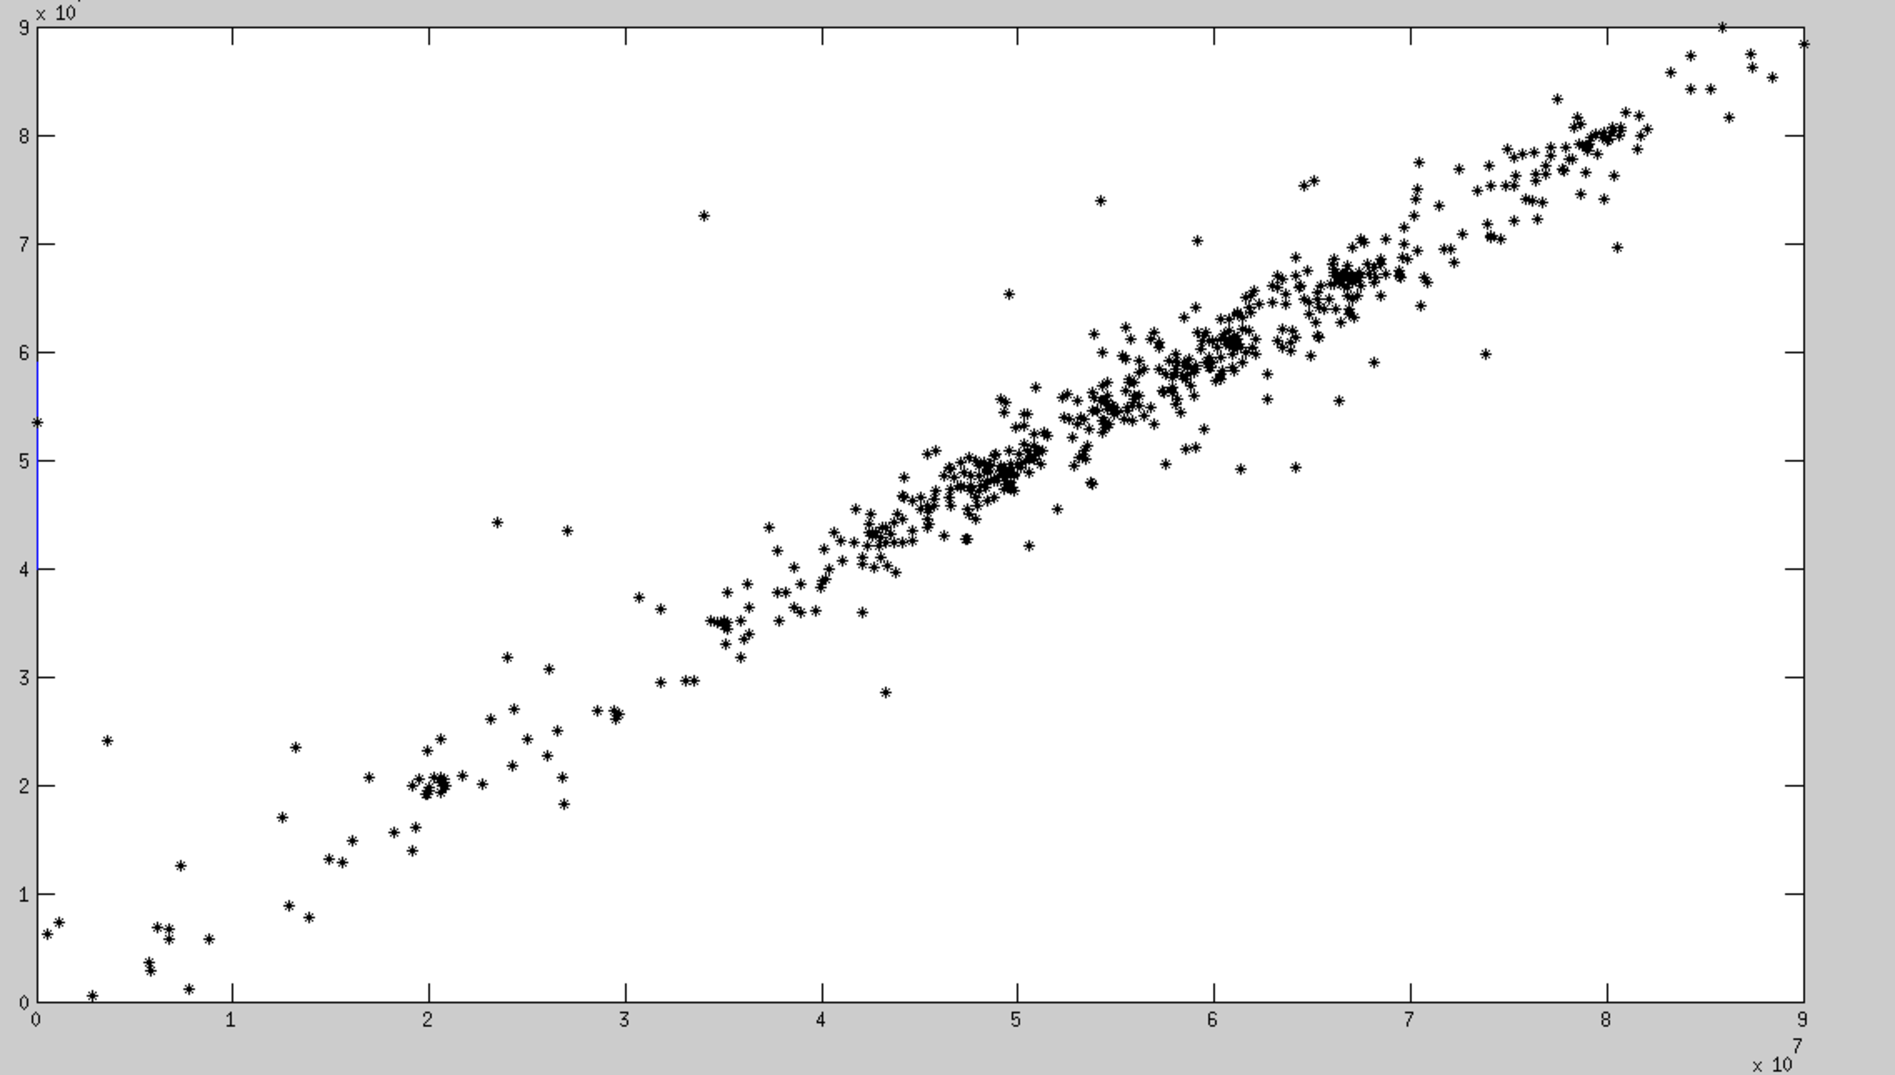
\includegraphics[width=2.5in]{salidaRBF.pdf}
	\caption{Salidas de la red RBF}
	\label{fig_mar}
\end{figure}
En el eje $x$ se pusieron las orientaciones otorgadas por el sistema de vision, y en el eje y se puso las salidas que nos da nuestro sistema de prediccion, por el grafico nos dijamos que las predicciones estan muy cercanas a los valores originales.
Para comparar nuestros resultados utilizamos una red Neuronal del tipo Focused Time Delay, esta tipo de red neuronal dinamica tiene la propiedad de volver a valores anteriores (\textit{delay}) para alimentar a las nuevas salidas, en este caso se dividio toda las muestras en partes para el entrenamiento, para la validacion y para las pruebas, a continuacion mostramos el la misma grafica(figura 5.3). En este caso el algoritmo fue implementado utilizando el  \textit{Neural Network Toolbox} del MatLab, el cual nos dio este resultado mostrado en la figura 5.3 :
\begin{figure}
	\centering
	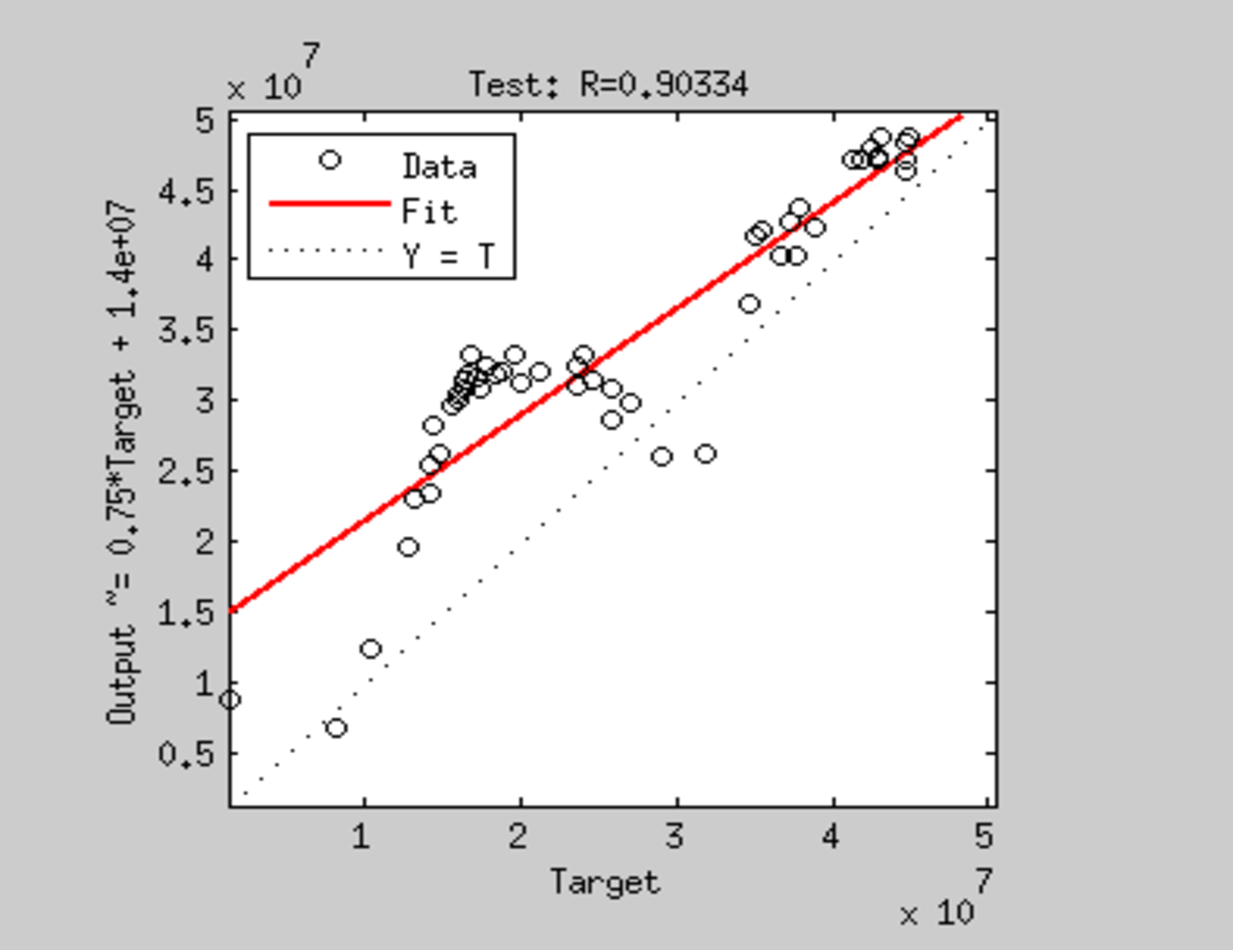
\includegraphics[width=2.5in]{salidaNAR.pdf}
	\caption{Salida de la Red Focused Time Delay}
	\label{fig_mar}
\end{figure}
